\documentclass[landscape]{article}

\usepackage{graphicx}
\usepackage{float}

\voffset = -90pt
\hoffset = -170pt
\textwidth = 700pt
\textheight = 550pt

\begin{document}

\thispagestyle{empty}

\begin{figure}[H]
  \centering
  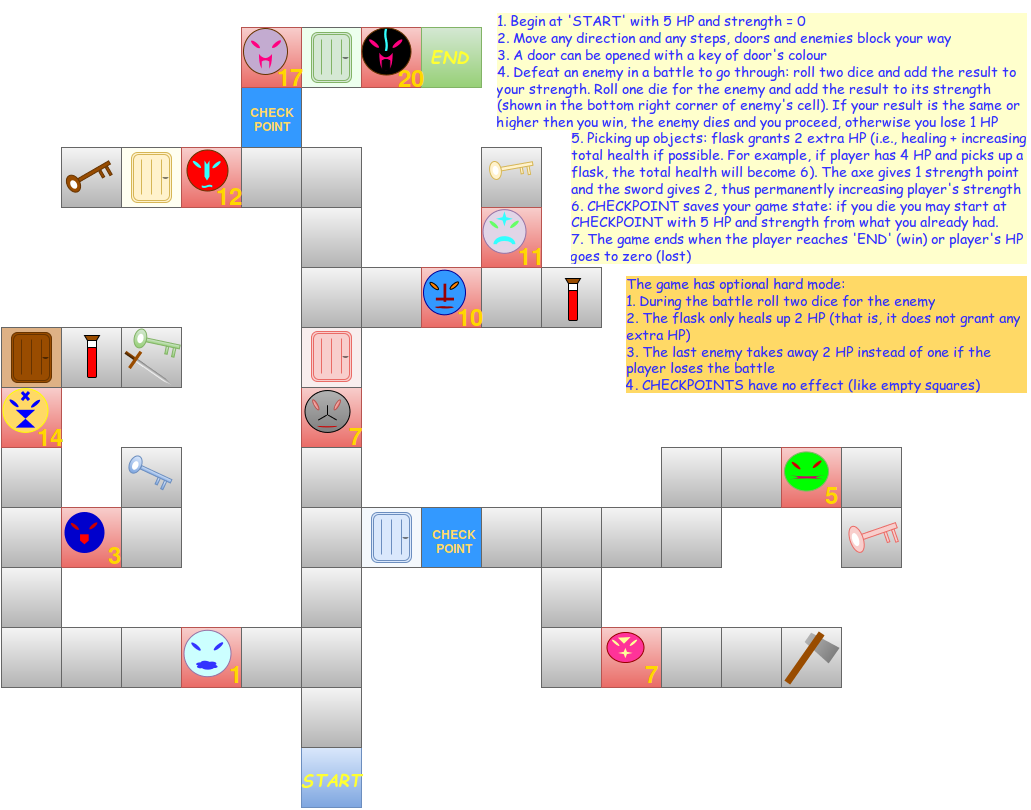
\includegraphics[height=\textheight]{simpleGameDesign3.png}
\end{figure}

\newpage

\subsubsection*{Feedback Influence}

From feedback I have extracted that rewarding the player with something more than
just reaching the exit might be more interesting.

After reading the feedback I have also devised a plan of adding check points to
help the players not to start from the beginning but from the last check point
they have visited.

\subsubsection*{Narrative}

You are an outlaw in a small settlement in a ravine surrounded with mountains.
The villagers have locked you in a barn for indefinite time. Recently the people
noticed that their sheep started to disappear and learned that the creatures
from one cave in the mountains are the reason. Few brave men went to the cave
and only one escaped. He told everyone about the unfortunate fate of his fellows
and how the monsters have made corridors in the cave with only one exit on the
other side of the cave.

After a brief discussion the village board has decided to offer you a chance to
clear your name and full support for the rest of your life if you agree to go
into the dreadful cave. You would wield a dagger, given leather clothes and your
task would be to clear the cave from the monsters and exit on the other side.

After considering your miserable situation you take their offer and approach the
entry of the cave together with several villagers. The people have given you a
torch and once you alone step inside they block the entry with a huge stone
which you cannot move. The only way for you is go pass through the cave.

The game tries to implement the writer---led narrative.

Once you are on a cross, you can choose a direction to continue.

If you see a door you may try to open it. If you have a key of the same colour
as the door then you can open, otherwise you would be given a hint to look for
the corresponding key.

If you see an enemy in front you will be offered to engage in a combat or to go
back and choose another direction. Apparently, you would have to fight most of
the monsters at some point, therefore, there will no sense in going back at that
point.

When you see an object on the space in front of you, you will be informed what
it looks like (a rusty axe, a blue key, a flask etc.). When you step on that
space you pick up the object and you are informed what happened (your strength
has permanently increased by one, you have got a blue key, you have healed
yourself for two hit points\dots).

Once you step on the check point square your game state is saved. That means, if
you die then you can start again from the check point if you want to, you HP
will be restored to five and the strength will be restored from what you had
when you stepped on the check point square. Note: in the hard mode the check
points square are inactive, no effect.

Winning state: once you step on the ``END'' square your character exits the cave
and goes to the village. People immediately perceive it as you succeeded (since
you survived and there was only one way to exit the cave) and praise. The
village board as promised gave you the house to live in and full support till
the end of your days, so you may choose to be lazy and do whatever you want.

Hard mode: the King of the country has heard about your heroic deeds and
granted you shining armour together with a skillfully crafted sword and offered
you to join his personal guards with a chance to participate in future great
adventures. You gratefully accept his offer and wait for new adventures.

\end{document}
